%---------------------------------------------------------------
% File information.

% Filename : docs/design.tex
% Purpose  : Multiplayer, networked Checkers game for CS451.
% Authors  : Corwin Belser <cmb539@drexel.edu>
%            Zach Brennan  < zab37@drexel.edu>
%            Kris Horsey   < kth37@drexel.edu>
%            Zach van Rijn < zwv23@drexel.edu>
% License  : MIT/X (excl. ext. libs; see respective licenses).
% Revision : 20170813

%---------------------------------------------------------------
% README.

% This is currently a DRAFT.
%
% Also please keep it to NO MORE THAN 64 columns. This isn't a
% requirement by LaTeX, but a guideline we are following for the
% entire project. Thanks.
%
% You will need some kind of LaTeX compiler. Recommend this:
% https://www.tug.org/texlive/acquire-netinstall.html
% which works on Windows and Linux.
%
% The `vhistory' package has nice documentation:
% http://mirrors.rit.edu\
% /CTAN/macros/latex/contrib/vhistory/doc/vh_sets_en.pdf
%
% And this page on making tables:
% https://en.wikibooks.org/wiki/LaTeX/Tables

%---------------------------------------------------------------
% Includes.

\documentclass[letterpaper]{article}

\usepackage{amssymb}                    % for keyword styling
\usepackage[english]{babel}
\usepackage{bookmark}                   % tracks .out files
\usepackage{cleveref}                   % \cref
\usepackage[usenames,dvipsnames]{color} % for colors
\usepackage{courier}                    % \ttfamily
\usepackage[useregional]{datetime2}
\usepackage{forest}                     % for directory tree
\usepackage{hyperref}                   % \url
\usepackage{listings}                   % \lstlisting, \lstset
\usepackage[numbers, square]{natbib}    % for proper \bibsection
\usepackage{rotating}                   % for sidewaysfigure
\usepackage{subcaption}                 % for nested figures
\usepackage{tabu}                       % flexible tables
\usepackage{tabulary}                   % \tabulary (more flex.)
\usepackage{tikz}                       % for dem ol' shapez!
\usepackage{vhistory}                   % for version history

\usetikzlibrary{shapes.geometric, arrows}

%---------------------------------------------------------------
% Shapes.

% Should probably come up with new shapes.

\tikzstyle{startstop} = [
    rectangle,
    rounded corners,
    minimum width=3cm,
    minimum height=1cm,
    text centered,
    draw=black,
    fill=red!30
]

\tikzstyle{io} = [
    trapezium,
    trapezium left angle=70,
    trapezium right angle=110,
    minimum width=3cm,
    minimum height=1cm,
    text centered,
    draw=black,
    fill=blue!30
]

\tikzstyle{process} = [
    rectangle,
    minimum width=3cm,
    minimum height=1cm,
    text centered,
    text width=3cm,
    draw=black,
    fill=orange!30
]

\tikzstyle{decision} = [
    diamond,
    minimum width=3cm,
    minimum height=1cm,
    text centered,
    draw=black,
    fill=green!30
]

% Arrows.

\tikzstyle{arrow} = [thick,->,>=stealth]
\tikzstyle{conns} = [thick,-,>=stealth]


%---------------------------------------------------------------
% Listings.

% https://tex.stackexchange.com/questions\
% /31328/how-to-typeset-data-structures

% define a pseudocode language
\lstdefinelanguage{algpseudocode}
{
    keywordstyle=[1]{\keywordstyle},
    keywordstyle=[2]{\operatorstyle},
    keywordstyle=[3]{\typestyle},
    keywordstyle=[4]{\functionstyle},
    identifierstyle={\identifierstyle},
    keywords=[1]{%
    begin,end,%
    program,procedure,function,subroutine,%
    while,do,for,to,next,repeat,until,loop,%
    continue,endwhile,endfor,endloop,%
    if,then,else,endif,%
    return},
    literate={-}{$-$}1 {^}{$^\wedge$}1
    {>}{{$>$\ }}1 {<}{{$<$\ }}1
    {>=}{{$\geqslant$\ }}1 {<=}{{$\leqslant$\ }}1 
    {:=}{{$\gets$\ }}1 {!=}{{$\ne$\ }}1 {<>}{{$\ne$\ }}1
    {->}{{$\;\to\;$}}1
    {&&}{{\keywordstyle and\ }}4 {{||}}{{\keywordstyle or\ }}3
    {;}{\hspace{0.2em};}2 {,}{\hspace{0.2em},}2,
}

% some macros to fine-tune styles
\newcommand\keywordstyle{\rmfamily\bfseries\upshape}
\newcommand\operatorstyle{\rmfamily\mdseries\upshape}
\newcommand\typestyle{\rmfamily\mdseries\upshape}
\newcommand\functionstyle{\rmfamily\mdseries\scshape}

\newcommand\identifierstyle{\rmfamily\mdseries\itshape}

\newcommand\addkeywords[1]{%
    \lstset{morekeywords=[1]{#1}}}

\newcommand\addoperators[1]{%
    \lstset{morekeywords=[2]{#1}}}

\newcommand\addtypes[1]{%
    \lstset{morekeywords=[3]{#1}}}

\newcommand\addfunctions[1]{%
    \lstset{morekeywords=[4]{#1}}}

\definecolor{Brown}{cmyk}{0,0.81,1,0.60}
\definecolor{OliveGreen}{cmyk}{0.64,0,0.95,0.40}
\definecolor{CadetBlue}{cmyk}{0.62,0.57,0.23,0}
\definecolor{gray}{cmyk}{0,0,0,0.5}

%---------------------------------------------------------------
% Macros.

% Produces a sexy table for pre- and post-conditions.
\newcommand{\prepost}[3]
{
    \begin{tabulary}{\linewidth}{L}
    \textbf{Precondition}:  \\#1\\
    \textbf{Action}:        \\#2\\
    \textbf{Postcondition}: \\#3\\
    \end{tabulary}
}

% This version can be used inside a table.
\newcommand{\relates}[3]
{
    \begin{tabulary}{\linewidth}{L}
    \textbf{Include}:    \\#1\\
    \textbf{Extend}:     \\#2\\
    \textbf{Depends On}: \\#3\\
    \end{tabulary}
}

% This can be used normally or inside-inside a table (?).
\newcommand{\relatez}[3]
{
    \textbf{Include}:    \\#1\\
    \textbf{Extend}:     \\#2\\
    \textbf{Depends On}: \\#3\\
}

% Plain inside a table.
\newcommand{\formfield}[2]
{
    \begin{tabulary}{\linewidth}{L}
    \textbf{#1}:\\#2
    \end{tabulary}
}

% Macro to render a `use case' table. This is split up into 3
% components because in LaTeX you can only have up to 9
% parameters. I will probably go to Hell for this.

\newcommand{\usecasea}[7]
{
    \newpage
    \def\arraystretch{1.35}
    \begin{tabular}{|*{4}{l|}}
    \hline
    \multicolumn{2}{|l}{
        \formfield{Use Case Name}{#1}} &
    \multicolumn{1}{|l}{
        \formfield{ID}{#2}} &
    \multicolumn{1}{|l|}{
        \formfield{Priority}{#3}} \\
    \hline
    \multicolumn{1}{|l}{
        \formfield{Primary Actor}{#4}} &
    \multicolumn{1}{|l}{
        \formfield{Source}{#5}} &
    \multicolumn{1}{|l}{
        \formfield{Use Case Type}{#6}} &
    \multicolumn{1}{|l|}{
        \formfield{Level}{#7}} \\
    \hline 
}
\newcommand{\usecaseb}[4]
{
    \multicolumn{4}{|l|}{
        \formfield{Interested Stakeholders}{#1}} \\
    \hline
    \multicolumn{4}{|l|}{
        \formfield{Brief Description}{#2}} \\
    \hline
    \multicolumn{4}{|l|}{
        \formfield{Goal}{#3}} \\
    \hline
    \multicolumn{4}{|l|}{
        \formfield{Success Measurement}{#4}} \\
    \hline
}
\newcommand{\usecasec}[9]
{
    \multicolumn{4}{|l|}{
        \prepost{#1}{#2}{#3}} \\
    \hline
    \multicolumn{4}{|l|}{
        \formfield{Relationships}{\relatez{#4}{#5}{#6}}} \\
    \hline
    \multicolumn{4}{|l|}{
        \formfield{Typical Event Flow}{#7}} \\
    \hline
    \multicolumn{4}{|l|}{
        \formfield{Assumptions}{#8}} \\
    \hline
    \multicolumn{4}{|l|}{
        \formfield{Implementation Constraints}{#9}} \\
    \hline
    \end{tabular}
}

%---------------------------------------------------------------
% Configuration.

\renewcommand{\thefootnote}{\arabic{footnote}}

\title{
    Console-Based Checkers Game\\
    Software Design Specifications
    \footnote{CS451:002 Group 2, Drexel University}
}

% \usepackage{authblk} causes problems with alignment, though it
% also allows us to properly include affiliations.. pick poison.
\author{
    Belser, C.\\
    \texttt{cmb923@drexel.edu}
    \and
    Brennan, Z.\\
    \texttt{zab37@drexel.edu}
    \and
    Horsey, K.\\
    \texttt{kth37@drexel.edu}
    \and
    van Rijn, Z.\\
    \texttt{zwv23@drexel.edu}
}

\date{\today}

%---------------------------------------------------------------
% Document begin.

\begin{document}

%---------------------------------------------------------------
% Header.

\maketitle

\begin{abstract}

This document is intended to be used in conjunction with the
provided \texttt{requirements.pdf} document. \textbf{Note:} this
document is \emph{Proprietary and Confidential}; duplication
or reproduction of any content herein must be explicitly granted
in writing.

\end{abstract}

%---------------------------------------------------------------
% Table of Contents.

\tableofcontents
\newpage

%---------------------------------------------------------------
% Revision History.

\begin{versionhistory}
    \vhEntry{0.90}
        {\date{\DTMdisplaydate{2017}{07}{30}{-1}}}
        {ZV}
        {created initial \LaTeX~version}
    \vhEntry{0.91}
        {\date{\DTMdisplaydate{2017}{08}{06}{-1}}}
        {KH}
        {added Glossary \& updated Game Logic}
    \vhEntry{0.92}
        {\date{\DTMdisplaydate{2017}{08}{06}{-1}}}
        {ZB}
        {updated Coding Conventions}
    \vhEntry{0.94}
        {\date{\DTMdisplaydate{2017}{08}{11}{-1}}}
        {ZV}
        {added Docker notes}
    \vhEntry{0.95}
        {\date{\DTMdisplaydate{2017}{08}{012}{-1}}}
        {ZB}
        {finished section 5.2 Networking Module}
    \vhEntry{0.96}
        {\date{\DTMdisplaydate{2017}{08}{013}{-1}}}
        {KH}
        {Updated Sections 3 and 5}
    \vhEntry{0.97}
        {\date{\DTMdisplaydate{2017}{08}{13}{-1}}}
        {CB}
        {Class tables, component descriptions, display
        elements}
    \vhEntry{0.98}
        {\date{\DTMdisplaydate{2017}{08}{13}{-1}}}
        {ZV}
        {use cases, graphics, discussion}
    \vhEntry{1.00}
        {\date{\DTMdisplaydate{2017}{08}{13}{-1}}}
        {All}
        {final team approval}
\end{versionhistory}
\newpage

%---------------------------------------------------------------
% Introduction.

\section{Introduction}
\label{sec:intro}

This document describes in detail all components of the Console-
Based Checkers Game implementation outlined at a high-level in
the provided \texttt{requirements.pdf} document. To recap, this
application is a software implementation of the popular board
game Checkers, otherwise known as Draughts.

\subsection{Purpose of Document}
\label{sec:intro_outline}

This document is to describe the implementation of the Console-
Based Checkers Game, as described in the Console-Based Checkers
Requirements document. This game is designed to be played by 
two people on separate computers, connected to each other over
a network.

\subsection{Document Scope}
\label{sec:intro_scope}

The scope of this document shall contain the following:

\begin{enumerate}
    \item Design and description of complete system architecture
    \item Listing and design of all subsystems, with further
          descriptions and potential algorithms and details of
          their interconnectedness
    \item Amendments, if necessary, describing any changes to
          to the design after it has been approved by the client
\end{enumerate}

In particular, we divide the implementation details into
distinct categories:

\begin{enumerate}
    \item \emph{Game logic} - represents the core logic of the
          game, including official rules, move validation, and
          other necessary checks to ensure the game is played in
          a fair and correct manner
    \item \emph{Server logic} - the code necessary to create a
          game session, to which clients can connect and play,
          as well as ``spectator'' clients, time permitting; the
          server logic is responsible for maintaining network
          connections to the clients, using the above
          \emph{game logic} to further validate moves
    \item \emph{Client logic} - the client logic will control
          any visualization, user input, output as well as
          \emph{game logic} to ensure the user is able to play
          the game; the client will be responsible for ensuring
          that it can connect to the server, and for handling
          any disruptions in the network connection gracefully
\end{enumerate}

By implementing these components, we will have achieved a base
level of functionality (minimum viable product) which should be
sufficient to satisfy the client's needs. Further refinements or
changes shall be made, described and agreed upon in writing,
following the completion of the initial development phase.

%--What's the difference between this and the glossary? -Zach B
%--Intro definitions clarify abbreviations, glossary is for
% words -- not everyone knows - everyone else

\subsection{Definitions, Acronyms, Abbreviations}
\label{sec:intro_definitions}

\begin{enumerate}
    \item \emph{VNC} - Virtual Network Computing; a graphical
          desktop sharing system which allows remote users to
          connect to and potentially control a system which has
          a graphical user interface (GUI). In the context of
          this application, a future addition could be a
          web-based client that may utilize VNC to simplify the
          development/porting process of bringing the native
          game to the web browser
    
    \item \emph{Boardstate} - The data structure that contains
          the current state of the board, and the locations of
          each piece
    
    \item \emph{Board} - Refers to the visual representation of
          the \emph{BoardState}
           
    \item \emph{Game} - A capitalized \textbf{Game} shall be
          used in place of the full name of Console-Based
          Checkers, where appropriate
\end{enumerate}

%---------------------------------------------------------------
% Use Cases.

%% NOTICE
% http://robotics.ee.uwa.edu.au
%/courses/design/examples/example_design.pdf
% pg. 9

\section{Use Cases}
\label{sec:cases}

\subsection{Actors}
\label{sec:cases_actors}

\subsubsection{Active Player}
\label{sec:cases_actors_active}

The \textbf{active player} is a player who is currently engaged
in a loop with the server while they attempt to choose a valid
move. Each time the user submits a move to the server it will
respond with a message either acknowledging the move and provide
the updated game state, or it will request that the user provide
another attempt at a valid move, in which case the user is
notified that their previous attempt was invalid.

\subsubsection{Waiting Player}
\label{sec:cases_actors_waiting}

The \textbf{waiting user} is simply the other ``main'' player
(the opponent) who is engaged with the first player in a game of
Checkers. This user must wait until it is their turn in order to
make a move.

\subsubsection{Spectator}
\label{sec:cases_actors_spectator}

A \textbf{spectator} is the \texttt{3..n} connected client, who
does not have any interactions with the server aside from the
initial connection or receiving of notifications. If any such
input is provided, the server will simply ignore the request(s).

\subsection{List of Use Cases}
\label{sec:cases_list}

\subsubsection{Active Player}
\label{sec:cases_list_active}

\begin{enumerate}
    \item receive current game state from the server %1a DONE
    \item request (again) current game state from the server %2a DONE
    \item receive passive message notification %3a DONE
    \item receive (blocking) message notification %4a DONE
    \item send tentative valid move sequence %5a DONE
    \item receive move validity confirmation or rejection %6a DONE
    \item resign from game %7a DONE
\end{enumerate}

\subsubsection{Waiting Player}
\label{sec:cases_list_waiting}

\begin{enumerate}
    \item receive current game state from the server %1b DONE
    \item request (again) current game state from the server %2b DONE
    \item receive passive message notification %3b DONE
    \item receive (blocking) message notification %4b DONE
    \item resign from game %7b DONE
\end{enumerate}

\subsubsection{Spectator}
\label{sec:cases_list_spectator}

\begin{enumerate}
    \item receive current game state from the server %1c DONE
    \item request (again) current game state from the server %2c DONE
    \item receive passive message notification %3c DONE
    \item receive (blocking) message notification %4c DONE
\end{enumerate}

\subsection{Use Cases}
\label{sec:cases_cases}

%% THESE COME FROM ABOVE; EACH POINT IS AN \item ...

%% BEGIN USE CASE
%\usecasea
%{a}{a}{a}
%{a}{a}{a}{a}
%\usecaseb
%{a}
%{a}
%{a}
%{a}
%\usecasec
%{a}{a}{a}
%{a}{a}{a}
%{a}
%{a}
%{a}
%% END USE CASE

% BEGIN USE CASE (1a)
\usecasea
{Receive Game State}{RGS}{critical}
{Active Player}{primary}{core}{overview}
\usecaseb
{All}
{This use case describes the critical function of the system
where the player receives the current game state from server}
{The client receives the current game state from the server}
{The client and server have the same (byte-for-byte) game state
representation, and the client renders the board correctly}
\usecasec
{The client is connected to the server}
    {The server sends the current board state to the client}
    {The client and server have identical copies of the state}
{n/a}
    {n/a}
    {n/a}
{Client ready -> Server send -> Client receive}
{The data is not corrupted during transmission}
{n/a}
% END USE CASE (1a)

% BEGIN USE CASE (1b)
\usecasea
{Receive Game State}{RGS}{critical}
{Waiting Player}{primary}{core}{overview}
\usecaseb
{All}
{This use case describes the critical function of the system
where the player receives the current game state from server}
{The client receives the current game state from the server}
{The client and server have the same (byte-for-byte) game state
representation, and the client renders the board correctly}
\usecasec
{The client is connected to the server}
    {The server sends the current board state to the client}
    {The client and server have identical copies of the state}
{n/a}
    {n/a}
    {n/a}
{Client ready -> Server send -> Client receive}
{The data is not corrupted during transmission}
{n/a}
% END USE CASE (1b)

% BEGIN USE CASE (1c)
\usecasea
{Receive Game State}{RGS}{critical}
{Spectator}{primary}{core}{overview}
\usecaseb
{All}
{This use case describes the critical function of the system
where the player receives the current game state from server}
{The client receives the current game state from the server}
{The client and server have the same (byte-for-byte) game state
representation, and the client renders the board correctly}
\usecasec
{The client is connected to the server}
    {The server sends the current board state to the client}
    {The client and server have identical copies of the state}
{n/a}
    {n/a}
    {n/a}
{Client ready -> Server send -> Client receive}
{The data is not corrupted during transmission}
{n/a}
% END USE CASE (1c)

% BEGIN USE CASE (2a)
\usecasea
{Request Game State from Server}{RGS}{critical}
{Active Player}{primary}{core}{overview}
\usecaseb
{All}
{This use case describes the critical function of the system
where the player requests the updated game state from server}
{The client receives the current game state from the server}
{The client and server have the same (byte-for-byte) game state
representation, and the client renders the board correctly}
\usecasec
{The client is connected to the server}
    {The server sends the current board state to the client}
    {The client and server have identical copies of the state}
{n/a}
    {n/a}
    {n/a}
{Client ready -> Server send -> Client receive}
{The data is not corrupted during transmission}
{n/a}
% END USE CASE (2a)

% BEGIN USE CASE (2b)
\usecasea
{Request Game State from Server}{RGS}{critical}
{Waiting Player}{primary}{core}{overview}
\usecaseb
{All}
{This use case describes the critical function of the system
where the player requests the updated game state from server}
{The client receives the current game state from the server}
{The client and server have the same (byte-for-byte) game state
representation, and the client renders the board correctly}
\usecasec
{The client is connected to the server}
    {The server sends the current board state to the client}
    {The client and server have identical copies of the state}
{n/a}
    {n/a}
    {n/a}
{Client ready -> Server send -> Client receive}
{The data is not corrupted during transmission}
{n/a}
% END USE CASE (2b)

% BEGIN USE CASE (2c)
\usecasea
{Request Game State from Server}{RGS}{critical}
{Spectator}{primary}{core}{overview}
\usecaseb
{All}
{This use case describes the critical function of the system
where the player requests the updated game state from server}
{The client receives the current game state from the server}
{The client and server have the same (byte-for-byte) game state
representation, and the client renders the board correctly}
\usecasec
{The client is connected to the server}
    {The server sends the current board state to the client}
    {The client and server have identical copies of the state}
{n/a}
    {n/a}
    {n/a}
{Client ready -> Server send -> Client receive}
{The data is not corrupted during transmission}
{n/a}
% END USE CASE (2c)

% BEGIN USE CASE (3a)
\usecasea
{Receive passive message notification}{RGS}{critical}
{Acting Player}{primary}{core}{overview}
\usecaseb
{All}
{This use case describes the function where the player
receives a message about their input from the server }
{The client receives information about the current game state from the server}
{The client has received their message from the server}
\usecasec
{The client is connected to the server}
    {The server sends a message to the client}
    {The client has received the message from the server}
{n/a}
    {n/a}
    {n/a}
{Client ready -> Server send -> Client receive}
{The data is not corrupted during transmission}
{n/a}
% END USE CASE (3a)

% BEGIN USE CASE (3b)
\usecasea
{Receive passive message notification}{RGS}{critical}
{Waiting Player}{primary}{core}{overview}
\usecaseb
{All}
{This use case describes the function where the player
receives a message about their input from the server }
{The client receives information about the current game state from the server}
{The client has received their message from the server}
\usecasec
{The client is connected to the server}
    {The server sends a message to the client}
    {The client has received the message from the server}
{n/a}
    {n/a}
    {n/a}
{Client ready -> Server send -> Client receive}
{The data is not corrupted during transmission}
{n/a}
% END USE CASE (3b)

% BEGIN USE CASE (3c)
\usecasea
{Receive passive message notification}{RGS}{low}
{Spectator}{primary}{core}{overview}
\usecaseb
{All}
{This use case describes the function where the player
receives a message about their input from the server }
{The client receives information about the current game state from the server}
{The client has received their message from the server}
\usecasec
{The client is connected to the server}
    {The server sends a message to the client}
    {The client has received the message from the server}
{n/a}
    {n/a}
    {n/a}
{Client ready -> Server send -> Client receive}
{The data is not corrupted during transmission}
{n/a}
% END USE CASE (3c)

% BEGIN USE CASE (4a)
\usecasea
{Receive (blocking) message notification}{RGS}{critical}
{Acting Player}{primary}{core}{overview}
\usecaseb
{All}
{This use case describes the function where the player
receives a message about their invalid input from the server }
{The client receives information about the current game state from the server}
{The client has received their message from the server}
\usecasec
{The client is connected to the server and makes an invalid move}
    {The server sends a message to the client}
    {The client has received the message from the server}
{n/a}
    {n/a}
    {n/a}
{Client ready -> Server send -> Client receive}
{The data is not corrupted during transmission}
{n/a}
% END USE CASE (4a)

% BEGIN USE CASE (4b)
\usecasea
{Receive (blocking) message notification}{RGS}{critical}
{Waiting Player}{primary}{core}{overview}
\usecaseb
{All}
{This use case describes the function where the player
receives a message about their invalid input from the server }
{The client receives information about the current game state from the server}
{The client has received their message from the server}
\usecasec
{The client is connected to the server and makes an invalid move}
    {The server sends a message to the client}
    {The client has received the message from the server}
{n/a}
    {n/a}
    {n/a}
{Client ready -> Server send -> Client receive}
{The data is not corrupted during transmission}
{n/a}
% END USE CASE (4b)

% BEGIN USE CASE (4c)
\usecasea
{Receive (blocking) message notification}{RGS}{low}
{Spectator}{primary}{core}{overview}
\usecaseb
{All}
{This use case describes the function where the player
receives a message about their invalid input from the server }
{The client receives information about the current game state from the server}
{The client has received their message from the server}
\usecasec
{The client is connected to the server and makes an invalid move}
    {The server sends a message to the client}
    {The client has received the message from the server}
{n/a}
    {n/a}
    {n/a}
{Client ready -> Server send -> Client receive}
{The data is not corrupted during transmission}
{n/a}
% END USE CASE (4c)

% BEGIN USE CASE (5a)
\usecasea
{Send Tentative Valid Move Sequence}{STVMS}{critical}
{Active Player}{primary}{core}{overview}
\usecaseb
{All}
{This use case describes the critical function of the system
where the client sends an expectedly valid move sequence
to the server}
{The server receives move sequences from clients}
{The server receives a move sequence from the client}
\usecasec
{The client gets a move sequence from the user}
    {The client sends the move sequence to the server}
    {The server receives the move sequence}
{n/a}
    {n/a}
    {n/a}
{Client Move Ready -> Server ready -> Client send ->
Server receive -> Server send -> Client receive}
{The data is not corrupted during transmission}
{n/a}
% END USE CASE (5a)

% BEGIN USE CASE (6a)
\usecasea
{Receive Move Validity Confirmation or Rejection}{RMVCR}{critical}
{Active Player}{primary}{core}{overview}
\usecaseb
{All}
{This use case describes the critical function of the system
where the client receives a validity response after sending
a move to the server}
{The client receives a validity response from the server}
{The client receives a confirmation for a valid move, and
a rejection for an invalid move}
\usecasec
{The client sends a move to the server}
    {The server sends the confirmation or rejection to the
    client}
    {The client receives and identifies the response}
{n/a}
    {n/a}
    {n/a}
{Server ready -> Client send -> Server receive -> Server send
-> Client receive}
{The data is not corrupted during transmission}
{n/a}
% END USE CASE (6a)

% BEGIN USE CASE (7a)
\usecasea
{Resign from the game}{RGS}{critical}
{Active Player}{primary}{core}{overview}
\usecaseb
{All}
{This use case describes the critical function of leaving the
game while it is in progress}
{The game ends, with the opponent declared the victor}
{Only one player remains connected, and a win-state is entered,
with that player declared the victor}
\usecasec
{Both players are connected to the server}
{The player drops connection, either intentionally or not}
{The game enters a win-state, and the opponent is declared the victor}
{n/a}
    {n/a}
    {n/a}
{Client disconnects -> Server recognizes lost connection -> Opponent wins}
{The server recognizes that the opponent has disconnected immediately}
{n/a}
% END USE CASE (7a)

% BEGIN USE CASE (7b)
\usecasea
{Resign from the game}{RGS}{critical}
{Waiting Player}{primary}{core}{overview}
\usecaseb
{All}
{This use case describes the critical function of leaving the
game while it is in progress}
{The game ends, with the opponent declared the victor}
{Only one player remains connected, and a win-state is entered,
with that player declared the victor}
\usecasec
{Both players are connected to the server}
{The player drops connection, either intentionally or not}
{The game enters a win-state, and the opponent is declared the victor}
{n/a}
    {n/a}
    {n/a}
{Client disconnects -> Server recognizes lost connection -> Opponent wins}
{The server recognizes that the opponent has disconnected immediately}
{n/a}
% END USE CASE (7b)

%---------------------------------------------------------------
% System Overview.

\section{System Overview}
\label{sec:overview}

\subsection{Description of Software}
\label{sec:overview_description}

This document describes the complete requirements for a console-
based implementation of the game \emph{Checkers}. Slight changes
may be present between the original game and the console-based
implementation (hereforth known as \textbf{game}). Therefore, it
is imperative that the product description be read, understood,
and any confusion clarified, by all parties, before development
begins.

The \textbf{game} is a two player game designed to be played
remotely (by two computers on joint or disjoint networks). When
a player joins the game they are taken to a waiting screen until
a second player has joined. Once two players are connected, they
are taken to a checker game board and begin the game. Players
then take turns making moves until either a stalemate is reached
(neither player can perform a move) or one player has no pieces
remaining on the board. At this point a winner is displayed (or
a draw in the case of a stalemate) and the game concludes.

\subsection{Technologies Used}
\label{sec:overview_technologies}

To aid in the development process, as well as provide a robust
deliverable, we make use of several technologies and software
libraries. Some of these are necessarily part of our design, and
others are only used during the development and build process.
In the latter case, it is possible to omit these components from
the deliverable.

\subsubsection{Docker}
\label{sec:overview_technologies_docker}

Docker~\cite{docker} is a software platform that abstracts many
aspects of the operating system in order to provide an isolated
environment, called a `container', which may contain only the
bare minimum required libraries and packages to support a given
application. The filesystem, network interfaces, and other parts
of the host system are available to the container as needed, and
while it shares a common kernel with other adjacent containers,
it does not depend on the host system for any other libraries.

Within the context of our Checkers implementation, Docker is
instrumental in providing consistent development and deployment
environments, reducing development time and costs by allowing us
to target one platform while supporting many. In particular, we
utilize a static build toolchain with which we compile static
binaries that can be distributed to and executed on almost any
similar platform. The ideal scenario is that the user(s) would
not need to deploy any build environment, compile any software,
or otherwise perform any potentially time-consuming steps, and
instead can simply copy a precompiled executable with which they
can run.

If this is not desirable, or in the event that changes are made
to the application source code or for security / trust concerns,
a new build environment can be constructed with a trivial amount
of work because this infrastructure is \emph{entirely scripted}.

Our usage of Docker is particularly interesting. Imagine the
following scenario:

\begin{enumerate}
    \item A Docker image \texttt{alpine:checkers} is created
          based on the \texttt{docker/Dockerfile} file in the
          project tree, containing all of the necessary tools
          and development libraries. This image is built using
          the command \texttt{make image} (which does some
          further processing).
    \item Any time a developer or user performs some action
          that requires this development environment, such as
          building the game, testing the source code, etc.,
          they spawn an ephemeral instance of the image,
          called a \emph{container}, which is run by default
          with a flag \texttt{--rm} which causes the container
          to be deleted when it is exited. Not to worry, the
          containers are designed to be temporary.
    \item As soon as a container is spawned, the main project
          directory is mounted inside the container to a
          configurable location. Inside the container, the
          user now has full access to the project source.
          However, instead of dropping the user into a shell,
          which is possible via the \texttt{make envir}
          command, the top-level \texttt{Makefile} executes
          various commands inside the container
          \emph{on behalf of} the user. The user doesn't even
          realize that these actions are being performed inside
          the container's consistent development environment.
    \item The developer (or user, if desired) can simply run
          \texttt{make game} or \texttt{make check} to either
          build the game's static executable(s), or check the
          source code and memory for errors. Because we mount
          the local source tree to the container instead of
          copying the source code or cloning it from the
          development repository, the static \texttt{x86\_64}
          executable is built directly into the \texttt{bin/}
          directory, ready for distribution.
\end{enumerate}

Our main \texttt{Makefile} operates in the manner outlined in
\cref{fig:overview_technologies_docker_makefile}.

\lstset{basicstyle=\ttfamily}
\lstset{frame=tb}
\begin{figure}
    \begin{lstlisting}
    $ make usage
    Usage:

      make <target>

    Targets:

      usage         prints this text then exits
      image         builds the devel. Docker img.
      envir         spawns/enters devel. envir.
      clean         remove intermediate files
      check         runs   various tests on code
      game          builds the Checkers(tm) game
      run-loc       runs   the game on this mach.
      run-con       runs   the game in Container
    \end{lstlisting}
    \caption{Primary \texttt{Makefile}}
    \label{fig:overview_technologies_docker_makefile}
\end{figure}

\subsubsection{Alpine Linux}
\label{sec:overview_technologies_alpine}

The primary Docker image that we will use is based off of Alpine
Linux~\cite{alpine}, a secure, minimal Linux distribution that
targets embedded systems and low-resource platforms in an effort
to maximize efficiency. For context, the minimal Alpine image is
just \texttt{5MB}, and it utilizes \emph{MUSL}~\cite{musl} and
\emph{BusyBox}~\cite{busybox} to provide efficient and correct
C/C++ libraries and standard utilities.

\subsubsection{ncurses}
\label{sec:overview_technologies_ncurses}

We make use of a software library \emph{ncurses}~\cite{ncurses}
for the implementation of our graphical user interface, which is
of course console-based, in other words running under a terminal
emulator such is standard practice today for most Unix-based
systems. In effect, many of the platform-specific changes that
we would need to support can be safely accounted for by relying
on \emph{ncurses} to handle these differences.

\subsubsection{VNC}
\label{sec:overview_technologies_vnc}

The software \emph{noVNC}~\cite{vnc} is a utility that enables
web-based connections to a VNC server, which is one way to share
a graphical display remotely over a network. This will enable us
to provide a web-based interface to our game in the event that
we cannot natively compile the application into
WebAssembly~\cite{webassembly}, which is to be determined.

%---------------------------------------------------------------
% Design Considerations.

\section{Design Considerations}
\label{sec:design}

Upon our client's request, we must develop a networked Checkers
implementation. This is not necessarily a problem per se, but by
choosing to implement the application in the C programming
language, we must be careful and thorough in providing a robust
deliverable. Our solution must account for unexpected network
troubles such as dropped packets or corrupted data.

As we are using Docker for our development and potentially the
execution environment, we make the guarantee that our software
will function correctly within this predefined environment, and
we aim to design our software to be compatible with external
platforms but cannot make such guarantees as to its efficacy. We
do not plan to develop for other platforms, but we will account
for the potential change of plan by allocating some slack time
to the matter.

\subsection{Assumptions and Dependencies}
\label{sec:design_assumptions}

In order to guarantee that the software builds and runs on an
agreed-upon generic platform, and operates correctly, we define
the minimum expected software and hardware configuration that
must be supported by the application. In other words, the game
should be playable with the minimum specifications, but it can
be assumed that most users will have machines that at least
meet or exceed the ``ideal'' hardware and/or software.

\begin{figure}
    \centering
    \begin{subfigure}{.50\textwidth}
        \centering
        \begin{tabular}{l*{2}{c}r}
            Component & Min.    & Ideal    \\
            \hline
            CPU       & 200 MHz & 1.0 GHz  \\
            Memory    &  64 MB  & 256 MB   \\
            Disk      & 500 MB  & 1.0 GB   \\
            Display   & 800x600 & 1024x768 \\
        \end{tabular}
        \caption{Hardware}
        \label{fig:design_assumptions_hard}
    \end{subfigure}%
    \begin{subfigure}{.50\textwidth}
        \centering
        \begin{tabular}{l*{2}{l}r}
            Component & Min.   & Ideal  \\
            \hline
            kernel    & 2.6.32 & 4.4.0  \\
            make      & 3.82   & 4.1    \\
            gcc       & 4.8.4  & 5.4.0  \\
            bash      & 4.2.46 & 4.3.48 \\
        \end{tabular}
        \caption{Software}
        \label{fig:design_assumptions_soft}
    \end{subfigure}
    \caption{Generic System Requirements}
    \label{fig:design_assumptions}
\end{figure}

\subsubsection{Hardware}
\label{sec:design_assumptions_hard}

\cref{fig:design_assumptions_hard} contains minimum and ideal
specifications of a generic platform that should be able to
operate the game. This does \emph{not} necessarily mean it needs
to be able to compile (build the game), but the ideal
specifications should be sufficient to do so.

\subsubsection{Software}
\label{sec:design_assumptions_soft}

\cref{fig:design_assumptions_soft} contains minimum and ideal
specifications of a generic platform that should be able to
operate the game. This does \emph{not} necessarily mean it needs
to be able to compile (build the game), but the ideal
specifications should be sufficient to do so.

\subsection{Dependencies}
\label{sec:design_dependencies}

Most or all of the software dependencies are directly satisfied
or satisfied by equivalent packages in the first stage of the
project prototype. These are bundled into the base Docker image
that we will use; all such discussion shall occur in separate
Docker-related documents, if applicable.

\subsection{General Constraints}
\label{sec:design_constraints}

To more comfortably fit our design and development of our
software into the time constraints imposed by our client, we
define a set of constraints on the project. In effect, detailing
further the project scope in areas not yet covered.

\subsubsection{End-User Environment}
\label{sec:design_constraints_1}

The \textbf{Game} is being developed with the intention of
running inside of Docker, so that the actual User Environment is
always controlled, and will function as expected. Thus there are
no constraints on the user system, other than an ability to run 
the Docker software.

\subsubsection{Availability and Volatility of Resources}
\label{sec:design_constraints_2}

The resources that are utilized for the project are all open
source and thus are available for anyone to use. These resources
are thus susceptible to being changed causing future releases of
the tools to no longer work with our program. Release version
specifications are contained in the requirements documentation. 

\subsubsection{Standards Compliance}
\label{sec:design_constraints_3}

The \textbf{Game} will meet all IEEE's standards for software of
this nature. 

\subsubsection{Interoperability}
\label{sec:design_constraints_4}

The \textbf{Game} will not have the ability to interact with
external programs or systems.

\subsubsection{Data Repository / Distribution}
\label{sec:design_constraints_5}

The data is currently hosted within a Git repository. Once the
project reaches completion, users will be able to find and
receive the code and documentation from a public portion of the
Git repository. The way users will run the code is through
Docker a platform agnostic program that will let user run to the
code on any machine that supports the program. 

\subsubsection{Verification, Validation, and Testing}
\label{sec:design_constraints_6}

We will utilize a unit-testing framework for the C language
called \emph{check}
\footnote{more details in \texttt{requirements.pdf}} and a
memory checking tool called \emph{valgrind} to ensure that our
code is safe and correct. Our top priority beyond implementing
all of the agreed-upon features is to do so without creating the
possible of a software, hardware, or network crash.

\subsubsection{Other Quality Controls}
\label{sec:design_constraints_7}

To maintain high quality software, after every major revision,
the group redoes all the testing for the sections to make sure
components that have been working, stay working as well and to
verify the status of previously nonworking portions of the
software. 

\subsection{Goals and Guidelines}
\label{sec:design_guidelines}

We aim to achieve the satisfaction of our client by providing
the highest quality service possible, focusing on the following
areas:

\begin{enumerate}
    \item The product must look, feel, and behave similarly to
          how a typical person would play the classic Checkers
          board game. This means, avoiding unnatural language or
          pop-up dialogs that could detract from the game
          experience.
    \item Since the players will be the bottleneck in the game,
          it is not critical to design for speed beyond being
          able to support the minimum hardware and software
          specifications outlined in
          \cref{sec:design_assumptions}.
\end{enumerate}

\subsection{Design Rationale}
\label{sec:design_rationale}

\subsubsection{Docker}
\label{sec:design_rationale_docker}

Our team has decided to make use of the Docker program because
it allows users on the range of operating systems from Windows,
macOS, and Linux to all be able to have an identical experience
when they are interacting with our Checkers program. Another
consideration is that with a singular platform testing can be
done much easier as their is no potential for unique errors to
appear.

\subsubsection{Separate Client/Server Modules}
\label{sec:design_rationale_client_server}

Our team has decided on implementing separate Client and Server
programs, as opposed to making a singular program that could
function as both Client and Server. This decision was made in
order to keep the codebase clean and concise. Another
consideration was the ease of use for the Player. They do not
need to have access to any of the Server functions, and giving
them more options to choose from, and making the game more
complex to set up, and less intuitive to use goes directly
against our outlined ideology for this system.

\subsubsection{1x32 Boardstate Storage}
\label{sec:design_rationale_boardstate}

There are many different ways to represent the boardstate, but
in the end, we chose to use a 1x32 array. In this array contains
a single \emph{Piece} in each space, and each index of the array
represents a single location on the board. There are 32 spaces
accessible by the pieces, which are numbered from left to right,
and top to bottoms, starting with 1, and going to 32. Keeping
the array this size allows us to avoid excessively long calls to
different 2D locations, and instead keep everything accessible
with a single integer index, which is much simpler and easier to
read. It also allows us to only use the minimum amount of
locations, so it is more difficult for a piece to get to
somewhere that it shouldn't be able to.

%---------------------------------------------------------------
% Architectural Strategies.

\section{Architectural Strategies}
\label{sec:strategies}

\subsection{Choice of Language}
\label{sec:strategies_language}

As a reasonable software engineering firm, our team has decided,
with the approval of our client, to implement our solution using
the C programming language. Grateful for the flexibility that
our client is giving us, we hope to gain a better understanding
of the tools, software libraries, and design principles involved
in using such a language, in that we can apply these techniques
and experiences to future work.

\subsection{Planning for Future Development}
\label{sec:strategies_future}

Our implementation of the Checkers game aims to be functionally
complete, with only minor possible future enhancements. We will
need to take into account the feasibility of porting our product
to mobile devices, web browsers, and potentially other platforms
but should not focus on creating an ideal one-size-fits-all
product.

\subsection{User Interface Paradigms}
\label{sec:strategies_ui}

Console-based games typically use a computer keyboard for input,
though may additionally accept mouse input. We will restrict our
product to accept only keyboard input. Common interfaces, or a
wrapper, could be written to make it easier to adapt the product
to accept other forms of user input, but this is outside of the
scope until further amendments to this document exist.

\subsection{Error Detection and Recovery}
\label{sec:strategies_recovery}

Due to the short-lived nature of a typical Checkers game session
we will avoid worrying about corrupted disks, memory, or other
hardware components. The critical aspect of our product is to
ensure that at least two connected clients (players) have a
seamless experience during their gameplay. As such, it is
imperative that we develop straightforward, clean, and robust
networking logic and code to handle any unforseen troubles
gracefully.

At the end of the day however, as this is not a mission-critical
application, we need not spend an unreasonable amount of effort
in this area if it means sacrificing the quality of other
portions of our product.

\subsection{Memory Management}
\label{sec:strategies_memory}

On a similar note as in \cref{sec:strategies_recovery}, our
product is not inherently a memory-intensive application, and
within our guaranteed Docker-based testing platform any memory
that is ``leaked'' is automatically cleaned up upon the
termination of the application. The third-party libraries we use
may also leak memory beyond our control.

We will make every reasonable effort to account for memory leaks
but cannot guarantee that our product will be free of memory
leaks.

\subsection{Concurrency and Synchronization}
\label{sec:strategies_concurrency}

We will employ a thread-based model to ensure that any remote
client is able to connect without the connection dropping due to
an unlikely but possible scenario where the server is processing
a previous request in that exact moment. By taking this approach
we can also accept, rather trivially, additional (third, fourth,
etc.) clients to serve as \emph{spectators}.

Outside of the networking module, concurrency need not be used.

\subsection{Containerization and Deployment}
\label{sec:strategies_deployment}

Deployment of our product (including, but not limited to testing
and automated builds, distribution of the compiled executable(s)
and other critical components of the software development
process) shall be guaranteed with a core set of constraints.

%---------------------------------------------------------------
% System Architecture.

\section{System Architecture}
\label{sec:architecture}

\begin{figure}
    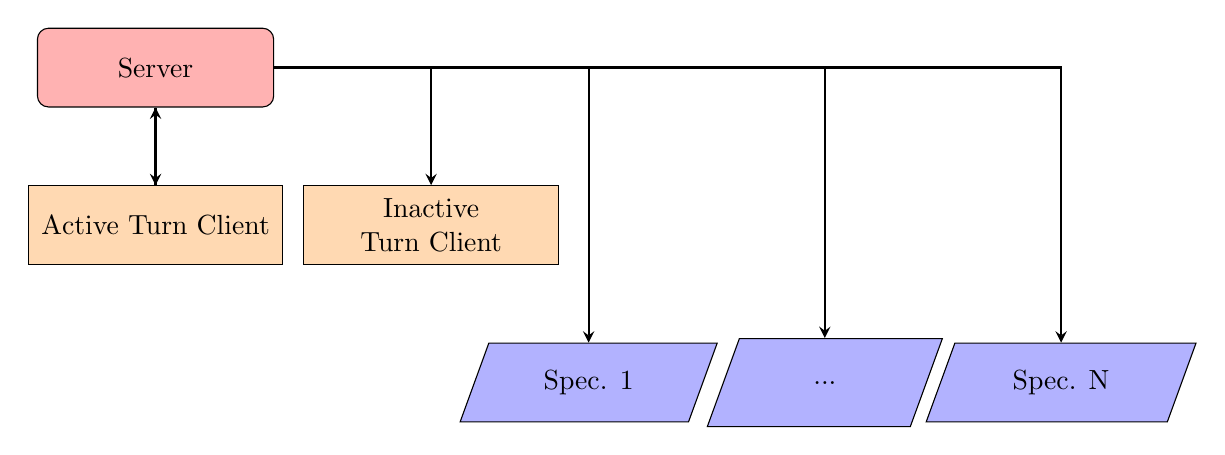
\begin{tikzpicture}[node distance=2cm]
    \node (server) [startstop] {Server};
    \node (client_a) [process, below of=server]
        {Active Turn Client};
    \node (client_b) [process, right of=client_a, xshift=1.5cm]
        {Inactive Turn Client};
    \node (spects_a) [io, right of=client_b, yshift=-2cm]
        {Spec. 1};
    \node (spects_b) [io, right of=spects_a, xshift=1cm]
        {...};
    \node (spects_c) [io, right of=spects_b, xshift=1cm]
        {Spec. N};

    \draw [arrow] (server) -- (client_a);
    \draw [arrow] (client_a) -- (server);
    \draw [arrow] (server) -| (client_b);
    \draw [arrow] (server) -| (spects_a);
    \draw [arrow] (server) -| (spects_b);
    \draw [arrow] (server) -| (spects_c);
    \end{tikzpicture}
    \caption{Server-Client Hierarchy, Spectators Optional}
    \label{fig:diagrams_sch}
\end{figure}

\cref{fig:diagrams_sch} shows an overview of the components
and their relation to one another. Details for each component
will be discussed further.

\subsection{Core Module}
\label{sec:architecture_system1}

The \emph{core module} of our product will be included in all
major components of the final deliverable(s), including but not
limited to: \emph{client}, \emph{server} modules. The purpose of
the \emph{core module} is to consolidate necessary elements and
to avoid code repetition, documentation redundancy, and reduce
the potential for future debugging troubles. The core module 
of Checkers will contain all game logic, graphical components,
and all logic that links the Server and Client modules. This is
to ensure that the program will remain in sync and in the case
that the program gets out of sync allow for easy correction to 
occur at that the time of the issue occurring. The primary role 
of the Server will be to serve as the mediator between the
clients and will serve as the final as the final confirmation in
making sure moves are being handled properly through the use of
the core module. The clients themselves will be the way the
players and spectators interact with and monitor the game board
respectively. For the players the core module does move
validation to show what moves they have available and handles
all of their inputs.

% @all, please ignore this part for now I'll clean it up soon ~Z
\lstset{
    language=C,                         % Code langugage
    basicstyle=\ttfamily,               % Code font, Examples: \footnotesize, \ttfamily
    keywordstyle=\color{OliveGreen},    % Keywords font ('*' = uppercase)
    commentstyle=\color{gray},          % Comments font
    numbers=left,                       % Line nums position
    numberstyle=\tiny,                  % Line-numbers fonts
    stepnumber=1,                       % Step between two line-numbers
    numbersep=5pt,                      % How far are line-numbers from code
    %backgroundcolor=\color{lightgray},  % Choose background color
    frame=none,                         % A frame around the code
    tabsize=4,                          % Default tab size
    captionpos=b,                       % Caption-position = bottom
    breaklines=true,                    % Automatic line breaking?
    breakatwhitespace=false,            % Automatic breaks only at whitespace?
    showspaces=false,                   % Dont make spaces visible
    showtabs=false,                     % Dont make tabls visible
    %columns=flexible,                   % Column format
    morekeywords={__global__, __device__}, % CUDA specific keywords
}

\begin{figure}
    % comment alignment needs work; not monospaced w/ italics
    \lstset{keepspaces=true}
    \begin{lstlisting}
    #define N_ROWS      8

    /* total pieces */
    #define N_PCES      ((N_ROWS - 2) * (N_ROWS / 2) / 2)

    typedef
    struct game_piece
    {
        int player : 1;
        int kinged : 1;
    } piece;

    typedef
    struct game_board
    {
        piece *board[N_ROWS][N_ROWS / 2];
    } board;
    \end{lstlisting}
    \caption{\texttt{board.h}}
    \label{fig:architecture_system1}
\end{figure}

\subsubsection{Requisite Libraries}
\label{sec:architecture_system1_part1}

Using Alpine Linux \texttt{3.6} as a base Docker image, several
additional packages are required in order to build the libraries
mentioned in the \texttt{requirements.pdf} document.

\lstset{basicstyle=\ttfamily}
\lstset{frame=tb}
\begin{figure}
    \begin{lstlisting}
    RUN apk update && apk add --no-cache \
        bash      \ # shell
        cmake     \ # build tool
        coreutils \ # provides 'nproc' for parallel builds
        g++       \ # C++ compiler
        gcc       \ # C   compiler
        make      \ # build tool
        sed       \ # for text replacement
        upx       \ # binary packer; not currently used
        vim       \ # text editor for debugging
        wget        # generic CLI web client
    \end{lstlisting}
    \caption{Primary \texttt{Fragment of \texttt{Dockerfile}}}
    \label{fig:architecture_system1_part1_req1}
\end{figure}

Once these dependencies are satisfied, we can build the following
libraries and tools, described in \texttt{requirements.pdf}:

\begin{itemize}
    \item ncurses-6.0
    \item check-0.11.0
    \item freetype-2.8
    \item valgrind-3.13.0
    \item cppcheck-1.79
\end{itemize}

\subsubsection{Game Logic}
\label{sec:architecture_system1_part2}

The \textbf{Game} will store the \emph{Boardstate} as a 1x32
array of pieces. This matrix represents the 32 spaces on the
standard checkerboard that are reachable by the pieces. By using
basic addition or subtraction (depending on the type of piece,
and which way it can move) we can calculate the locations that
each piece can move to, and where they are able to jump to. This
allows us to take that information, and compare it with the
current \emph{Boardstate}, to generate all of the available
moves for each piece. In order to do this efficiently, we take
the index ($i$) of the piece that we want to check for moves on,
and perform $i \% 8$. 

This is done because there are 2 distinct row types; those that
start with a blank space on the board, and those that start with
an occupied space. Luckily, the first two rows represent both of
these types, and therefore can be used as a basis to calculate
moves for the rest of the board as well. We know that a piece
$j$ in the first row can move to either $j+4$ or $j+5$, and a
piece $k$ in the second row can move to either $k+3$ or $k+4$.
Using this information, we can add these integers to the
original indices, before modulation, to obtain the moves
available for any space on the board. For moving in the other
direction, the same method is used, but the distances for the
first row are $-3$ and $-4$, and for the second row are $-4$ and
$-5$.

After the possible moves are found, the game checks which pieces
are in each space that the selected piece can move to, and
determines whether or not it is able to make that move, in the 
current gamestate. 

\begin{sidewaysfigure}
    \centering
    \includegraphics[
        width=\textwidth,
        height=\textheight,
        keepaspectratio
    ]{img/UML_Game_Manager.png}
    \caption{Game Manager}
    \label{fig:architecture_system1_part2_manager}
\end{sidewaysfigure}

The way that jumps work, is by first finding the available moves
and then taking the available move in the same direction as the
first move. The game will then check the first move location to
see if it contains a jump-able piece, and then the final jump
location to confirm that it is empty.

% The game recognizes each piece as a value in an 12x12 matrix
% that utilizes the rows and columns 2-9 to avoid out of bounds
% issues. Each individual piece is assigned a color value either
% red or white, a status value either standard or king and board
% location that is row then column representation of where they
% are located. The way the game handles movement is standard red
% pieces start at the top of the board and can only move downward
% while white pieces start at the bottom of the board and can only
% move upward. When a standard piece promotes to a king they can
% now move in either direction on any move. Promotion for red
% pieces occur when their location places them in row 9 and for
% white pieces when they are in row 2. The way the game determines
% legal moves is that it checks each piece of the current player
% to see if they can make moves. The game determines this by
% looking to see if an adjacent space is empty. If a spot is
% adjacent and in a legal direction the system will return that it
% is a valid move. If an adjacent space is occupied by an opposing
% piece the system will check the next adjacent space in that
% direction. If that space is also empty then the user will be
% able capture that piece. The user must make one of the available
% capture moves. If a user tries to confirm an illegal move then
% the system will inform the move is illegal.

\subsection{Networking Module}
\label{sec:architecture_system2}

% ZACH B: DO THIS
% Did this -Zach B
% A wild Corwin appears
% Corwin uses UML! It's super effective.
The \texttt{Networking} module contains all functionality
required for the client and server applications to communicate
with each other. This includes methods for establishing and
closing connections, as well as the sending and receiving of
messages.

\begin{figure}
    \centering
    \includegraphics[
        width=\textwidth,
        height=\textheight,
        keepaspectratio
    ]{img/UML_Network.png}
    \caption{Network Module}
    \label{fig:architecture_system2_network}
\end{figure}

\begin{center}
\begin{tabu} to \textwidth {|X[l]|X[l]|}
\hline
\multicolumn{2}{|c|}{network.h} \\
\hline
connect\_to\_server(int port): int &
Connects to an existing server using the provided port.\\
\hline
connect\_to\_client(int port): int &
Accepts a connection request from a client using the provided
port.\\
\hline
send\_client\_msg(int conn\_id, client\_msg message): void &
Sends a \texttt{client\_msg} to the server associated with the
\texttt{conn\_id}.\\
\hline
send\_server\_msg(int conn\_id, server\_msg message): void &
Sends a \texttt{server\_msg} to the client associated with the
\texttt{conn\_id}.\\
\hline
receive\_client\_msg(int conn\_id, client\_msg message): void &
Accepts a \texttt{client\_msg} from the server associated with
the \texttt{conn\_id}.\\
\hline
receive\_server\_msg(int conn\_id, server\_msg message): void &
Accepts a \texttt{server\_msg} from the client associated with
the \texttt{conn\_id}.\\
\hline
\end{tabu}
\end{center}

\subsection{Server Module}
\label{sec:architecture_system3}

The \texttt{Server} module contains all functionality required
to interface with multiple clients, manage a master
\emph{Boardstate}, and ensure that the game is played without
error, according to the rules detailed in the requirement
document. This module will be broken down into three main
components:

\subsubsection{Network Communication Component}
\label{sec:architecture_system3_Comm}

This component will provide all functionality required to accept
communications from multiple clients, and place them into a game
together. It will also handle sending and receiving
\emph{sequences of moves} from the clients that are in the game,
and sending \emph{Boardstates} and messages to these clients, to
communicate necessary actions with the Players.

\subsubsection{Game Logic Component}
\label{sec:architecture_system3_logic}

This component will manage the \textbf{Game}, including the
storage of the \emph{BoardState}, and validation of Player
moves. This will contain all of the functionality required to
validate moves given to it by the Client. Although the Player
will only be able to select from a list of available moves that
are pre-validated by the Client, re-validating these moves on
the Server allows us to make sure that everything is
synchronized between the Players, and adds a security measure
against any possible cheating.

\begin{figure}
    \centering
    \includegraphics[
        width=\textwidth,
        height=\textheight,
        keepaspectratio
    ]{img/UML_Server.png}
    \caption{Server Module}
    \label{fig:architecture_system3_server}
\end{figure}

\begin{center}
\begin{tabu} to \textwidth {|X[l]|X[l]|}
\hline
\multicolumn{2}{|c|}{game\_logic.h} \\
\hline
is\_valid\_move(board board, move[] move): bool &
Evaluates a sequence of moves against the board. \texttt{move}
will contain a single move in the case of a normal move, and a
sequence of moves in the case of a sequence of one or more
jumps.\\
\hline
get\_possible\_moves(board board, bool player): move[] &
Evaluates each piece of the provided player for available moves,
returning a list of all $1^{st}$ generation moves. If a jump can
be made, only jumps will be returned.\\
\hline
get\_possible\_move(board board, piece piece, bool only\_jumps):
move[] &
Evaluates all moves an individual piece can make. If
\texttt{only\_jumps} is \texttt{true}, then only moves
consisting of a jump are returned.\\
\hline
\end{tabu}
\end{center}

\begin{figure}
    \centering
    \includegraphics[
        width=\textwidth,
        height=\textheight,
        keepaspectratio
    ]{img/UML_Game_State.png}
    \caption{Game State Module}
    \label{fig:architecture_system3_state}
\end{figure}

% @all, please ignore this part for now I'll clean it up soon ~Z
\lstset{
    language=C,                         % Code langugage
    basicstyle=\ttfamily,               % Code font, Examples: \footnotesize, \ttfamily
    keywordstyle=\color{OliveGreen},    % Keywords font ('*' = uppercase)
    commentstyle=\color{gray},          % Comments font
    numbers=left,                       % Line nums position
    numberstyle=\tiny,                  % Line-numbers fonts
    stepnumber=1,                       % Step between two line-numbers
    numbersep=5pt,                      % How far are line-numbers from code
    %backgroundcolor=\color{lightgray},  % Choose background color
    frame=none,                         % A frame around the code
    tabsize=4,                          % Default tab size
    captionpos=b,                       % Caption-position = bottom
    breaklines=true,                    % Automatic line breaking?
    breakatwhitespace=false,            % Automatic breaks only at whitespace?
    showspaces=false,                   % Dont make spaces visible
    showtabs=false,                     % Dont make tabls visible
    %columns=flexible,                   % Column format
    morekeywords={__global__, __device__}, % CUDA specific keywords
}

\begin{figure}
    % comment alignment needs work; not monospaced w/ italics
    \lstset{keepspaces=true}
    \begin{lstlisting}
    #define MAX_MOVE    12

    typedef
    struct coordinate
    {
        int row;
        int col;
    } coord;

    typedef
    struct game_move
    {
        coord from;
        coord dest;
    } move;

    typedef
    struct move_sequence
    {
        move moves[MAX_MOVE];
    } mseq;
    \end{lstlisting}
    \caption{\texttt{move.h}}
    \label{fig:architecture_system3_move}
\end{figure}

\subsection{Client Module}
\label{sec:architecture_system4}

The \texttt{Client} module contains all functionality required
to interface with the player, and relay content to and from the
server. This module will be further broken down into four main
components:

\subsubsection{Graphical Display Component}
\label{sec:architecture_system4_GUI}

This component will provide the functionality to display
information to the user. It will use the \textit{ncurses}
library to create a visualization of the \emph{Boardstate},
and show messages from the Server.

\begin{center}
\begin{tabu} to \textwidth {|X[l]|X[l]|}
\hline
\multicolumn{2}{|c|}{display.h} \\
\hline
initialize(): void &
Configures the terminal to \texttt{ncurses} display mode.\\
\hline
close(): void &
Frees the terminal from \texttt{ncurses} display mode.\\
\hline
draw\_board(board board): void &
Renders the board to the screen.\\
\hline
display\_msg(string msg, bool is\_blocking): void &
If \texttt{is\_blocking} is true, renders the message as a
popup over the board, requiring the enter key to dismiss. If
\texttt{is\_blocking} is false, renders the message at the
top of the window, over any previous message.\\
\hline
toggle\_highlight(piece piece): void &
renders or de-renders an inner border on the space containing
the piece.\\
\hline
toggle\_blink(piece piece): void &
Renders or de-renders an inner blinking border on the space
containing the piece.\\
\hline
\end{tabu}
\end{center}

\subsubsection{Player Input Component}
\label{sec:architecture_system4_Input}

This component will provide the functionality required to 
receive input from the Player, in order to play the
\textbf{Game}. This includes the logic behind the selection of
moves that are generated from the \textbf{Move Assistance}
component.

\begin{center}
\begin{tabu} to \textwidth {|X[l]|X[l]|}
\hline
\multicolumn{2}{|c|}{user\_interface.h} \\
\hline
\hline
key\_press: enum &
Enum for the possible keys the user may press to advance the
game.\\
\hline
\hline
get\_user\_choice(move[] moves): move &
Utilizes the \texttt{get\_selection} method to get the initial
piece of a move. Repeats this process to get the destination of
the move.\\
\hline
get\_key\_press(): key\_press &
Helper method to get keyboard input from the user.\\
\hline
get\_selection(piece[] choices): piece &
Displays available pieces the player may move, allowing the
player to use the \texttt{left} and \texttt{right} arrow keys to
change the selected piece, until the user confirms with the
\texttt{enter} key. Upon confirmation, the selected move is
returned.\\
\hline
\end{tabu}
\end{center}

\subsubsection{Move Assistance Component}
\label{sec:architecture_system4_Assist}

This component will contain all the necessary features to
determine which moves and jumps the Player can (or must) make.

\begin{center}
\begin{tabu} to \textwidth {|X[l]|X[l]|}
\hline
\multicolumn{2}{|c|}{game\_manager.h} \\
\hline
\hline
board: board &
Stores the current \texttt{BoardState}\\
\hline
player: bool &
Identifies which player the client is playing\\
\hline
\hline
get\_move(): move[] &
Utilizes \texttt{game\_logic} and \texttt{user\_interface}
components to generate possible moves and get user's selection\\
\hline
apply\_move(board board, move[] move): void &
Applies the given move sequence to a board.\\
\hline
update\_board(board board): void &
Updates the stored \texttt{BoardState} with the provided board\\
\hline
\end{tabu}
\end{center}

\subsubsection{Network Communication Component}
\label{sec:architecture_system4_Comm}

This component will handle all interaction between the Client
and Server modules. This will include receiving Boardstates,
sending pre-validated moves, and receiving messages for the
Player to view.

%---------------------------------------------------------------
% Policies and Tactics.

\section{Policies and Tactics}
\label{sec:policies}

\subsection{Choice of Compiler}
\label{sec:policies_compiler}

In accordance with the minimum software specifications outlined
in \cref{fig:design_assumptions_soft}, we can make certain
guarantees about the tools required to build our product. Using
the Docker platform to provide a consistent build environment,
we assert that we will prioritize support for the GNU C Compiler
(GCC) using a certain set of compiler flags and standards.

\lstset{basicstyle=\ttfamily}
\lstset{frame=tb}
\begin{figure}
    \begin{lstlisting}
    # In this case, $CC is the default inside container;
    # configured within the Dockerfile, if desired.

    # FLAG - linker options (use static and PIC)
    # LIBS - required link line to build the project

    FLAG := -static -fPIC -flto
    LIBS := -lncurses -lmenu -lc

    game:
        $(Q)$(RUNNER) \
            -v $(PROJECT_ABS):$(MOUNTS) \
            -it $(IMAGES) \
            $(CC) $(FLAG) \
            -o $(MOUNTS)/$(OUTFILE) \
            $(SRCFILE) \
            $(LIBS)
    \end{lstlisting}
    \caption{Game \texttt{Makefile} Target}
    \label{fig:policies_compiler_game_target}
\end{figure}

\subsection{Coding Conventions}
\label{sec:policies_conventions}

Naming Conventions:\\
    \begin{itemize}
    \item Constants in all capital letters
    \item Underscores to delimit words in struct, function,
          and variable names
    \item Pointers will be declared with the * near the
          variable name, and not the pointer type
    \item Global variables will be prepended by a 'g\_'
    \end{itemize}
Commenting standards:\\
    \begin{itemize}
    \item All functions will have a comment describing the
          input, output, and any parameters that are being
          passed in
    \item Comments will be placed with any code that may not be
          immediately obvious in their functionality
    \end{itemize}
Overall formatting guidelines:
    \begin{itemize}
    \item Code will be kept to 72 char width max
    \item Braces will done in the Allman style~\cite{allman}.
          This style puts the brace associated with a control 
          statement on the next line, indented to the same 
          level as the control statement. Statements within
          the braces are indented to the next level
    \item Four(4) spaces will be used as a level of indentation
    \item Global variables will be avoided
    \item All If, While, and Do statements will use braces,
          even if there is only a single line in the braces
    \item There will be a single space between keywords 
          (such as If, and While) and parentheses
    \item Constants shall be placed on the left side of 
          equalities and inequalities
    \item Each line shall contain one statement
    \item Each variable declaration will have it's own line
    \end{itemize}
    
\subsection{Source Code Organization}
\label{sec:policies_organization}

The source code is organized as shown in \cref{fig:source_code_org_tree}

%--Source Code Tree taken from Linux 'tree -d' command run on
%--the git repo 
%--on August 12, 2017 at 2:40pm.
\begin{figure}
\begin{forest}
  for tree={
    font=\ttfamily,
    grow'=0,
    child anchor=west,
    parent anchor=south,
    anchor=west,
    calign=first,
    edge path={
      \noexpand\path [draw, \forestoption{edge}]
      (!u.south west) +(7.5pt,0) |- node[fill,inner sep=1.25pt]
        {} (.child anchor)\forestoption{edge label};
    },
    before typesetting nodes={
      if n=1
        {insert before={[,phantom]}}
        {}
    },
    fit=band,
    before computing xy={l=15pt},
  }
[CS451-Checkers
  [docker]
  [docs
    [cleveref]
    [datetime2
      [samples]
    ]
    [hyperref
      [doc]
      [test]
    ]
  ]
  [spec]
  [src
    [fonts]
    [game]
    [network
     [common]
     [client]
     [server]
    ]
  ]
]
\end{forest}
\caption{Source Code Organization Tree}
\label{fig:source_code_org_tree}
\end{figure}

\subsection{Issue Tracking}
\label{sec:policies_issues}

Using GitLab for our repository gives us the ability to use the
built-in issue tracking system. This system allows us to create
Issue tickets, that contain a title and description, to fully
document the issue that is observed, and allow others to recreate
the issue for testing purposes. These tickets can be assigned
to a specific person on the team, or left open for anyone to
work on, as they are available. A "Due Date" is also able to 
be set, for critical systems that needed to be fixed by a 
certain time. Once a ticket is submitted, it is available to 
view by everyone associated with the project, and can be placed 
into a "To Do" or "Doing" list, depending on the current status
of the issue. 

While Issues are still open, it is possible for other members of
the project to leave a comment on the ticket, so that the team 
can collaborate on fixing the issues, without everyone having to
work on it at the same time.

From the Issue screen, a merge request can be created, so that 
the code to fix the problem is directly associated with the 
ticket, and easy to search for. Once the problem is fixed, the 
ticket is closed, and placed on the "Closed" list, where it is 
still available to view. This allows us to keep a log of what 
went wrong, how it was fixed, and the exact code that was used 
to fix it.

\subsection{Unit Testing}
\label{sec:policies_units}

The methodology behind our tests is treating every board
interaction like it is occurring on a physical checkerboard. The
goal is to test every situation that a player can expect to find
themselves in a standard game of checkers, as well as any
situations that occur specifically when someone is playing a
virtual game of checkers like a player trying to move pieces off
the virtual game board or leaving the game idle for extended
periods of time. The way we can ensure that the tests are good
is by making sure that we do identical tests that are completely
equivalent for both players to make sure we don't run into a
case where one player can do something the other player would be
unable to do. 

\subsection{Continuous Integration}
\label{sec:policies_integration}

The way that the we are automating testing is by creating
different board states in separate files for testing. By
utilizing these files, the group will be able to see what items
are currently working and  which are currently broken through
our unit testing. 

\subsection{Build Instructions}
\label{sec:policies_building}

Simply run the command listed in
\cref{fig:policies_building_game}.

\lstset{basicstyle=\ttfamily}
\lstset{frame=tb,showstringspaces=false}
\begin{figure}
    \begin{lstlisting}
    $ make game
    make[1]: Entering directory `/CS451-Checkers/docker'
    sudo docker run --rm \
            -v /CS451-Checkers:/home \
            -it alpine:checkers \
            cc -static -fPIC -flto \
            -o /home/./bin/out \
            ./src/fonts.c ./src/main.c ./src/game.c \
            -lncurses -lmenu -lc
    [sudo] password for me:
    make[1]: Leaving directory `/CS451-Checkers/docker'
    \end{lstlisting}
    \caption{Game \texttt{Makefile} Target}
    \label{fig:policies_building_game}
\end{figure}

%---------------------------------------------------------------
% Miscellaneous.

\section{Miscellaneous}
\label{sec:detail}

Most of the components within \cref{sec:architecture} should be
discussed in more detail, which may include additional low-level
subcomponents. This section will provide additional details
and/or follow-up discussion on these matters.

% \subsection{Classification}
% \label{sec:detail_classification}

% \emph{TODO: the kind of component, such as subsystem or module,
% class, package, function, file, etc}.

% \subsection{Definition}
% \label{sec:detail_definition}

% \emph{TODO: the specific purpose and meaning of the component,
% and it's OK to refer to the \texttt{requirements.pdf} document}.

% \subsection{Responsibilities}
% \label{sec:detail_responsibilities}

% \emph{TODO: responsibilities/behavior of each component; the
% goal here is to design a modular system that is loosely
% coupled like most CS majors :P}.

% \subsection{Constraints}
% \label{sec:detail_constraints}

% \emph{TODO: this should be lower-level constraints, including
% pre- and post-conditions (things that we can unit-test) and so
% forth}.

% \subsection{Uses / Interactions}
% \label{sec:detail_interactions}

% \emph{TODO: might be OK to remove this section unless anyone
% can think of good content to put here}.

% \subsection{Resources}
% \label{sec:detail_resources}

% \emph{TODO: this is not about memory/cpu limitations, but should
% discuss race conditions, deadlocks, and other awful situations
% that could prevent the product from working correctly}.

% \subsection{Processing}
% \label{sec:detail_processing}

% \emph{TODO: good idea to discuss the details of the setup and
% teardown of the server, client, and other things involved. Think
% like ``what happens when you go to google.com?'' at all layers}.

% \subsection{Interface / Exports}
% \label{sec:detail_exports}

% \emph{TODO: definitely describe the data structures used, how
% the server works, and DO CITE THE SOURCE CODE not paste here}.

% \subsection{TODO: SUBSYSTEM DESIGN}
% \label{sec:detail_system1}

% \emph{TODO: this is kind of a catch-all for details about other
% subsystems which were not fully described elsewhere}.
\subsubsection{Board Display}

\begin{figure}
    \centering
    \begin{subfigure}{.4\textwidth}
        \centering
        \includegraphics{img/piece120.png}
        \caption{Piece}
        \label{fig:ui_pieces_piece}
    \end{subfigure}
    \begin{subfigure}{.45\textwidth}
        \centering
        \includegraphics{img/crown120.png}
        \caption{Crown}
        \label{fig:ui_pieces_crown}
    \end{subfigure}
    \caption{Checkers Piece Design}
    \label{fig:ui_pieces}
\end{figure}

The checker pieces are 13 pixels wide, by 6 pixels tall (keeping
in mind that the rows of a terminal window are twice the size of
the columns). \cref{fig:ui_pieces} shows the design of the
basic and \texttt{Kinged} pieces. Given these sizes, the board
size can be calculated. There will be a one pixel border around
the edge of the window. The top row will be reserved for the
display of messages. Therefore the terminal size needed to
display the \textbf{Game} is \texttt{106px by 102px}.

\begin{figure}
    \centering
        \includegraphics[
        width=\textwidth,
        height=\textheight,
        keepaspectratio
    ]{img/logo.png}
    \caption{Game Logo}
    \label{fig:ui_logo}
\end{figure}

%---------------------------------------------------------------
% Glossary.

\newpage

\section{Glossary}
\label{sec:glossary}

Below is a comprehensive list of some of the terms and language
that we use within this document, knowledge of which will lead
to a more effective understanding of our product's design and
aid in future communications regarding our product.

\begin{itemize}
    \item \textbf{Checkerboard} NxN (typically 8x8) game board
          composed of alternating black/red (or other) squares
          on which game pieces \emph{Checkers} reside
    \item \textbf{Piece} standard Checkers disc with limited
          movement, specifically only forward-diagonal motion
    \item \textbf{King} Checkers piece that can move along any
          diagonals, forward or backward
    \item \textbf{Move} the act of changing the location of a
          piece on the board when it is that player's turn
    \item \textbf{Jump} the act of removing an opposing player's
          piece from the board, occurring in a straight diagonal
          fashion -- e.g., "hopping over" the opponent
    \item \textbf{Crowning}, the act of changing a standard
          game piece to a \emph{King}
\end{itemize}

\newpage

%---------------------------------------------------------------
% References.

%\addcontentsline{toc}{chapter}{References}
\renewcommand{\bibsection}{\section{\refname}} % uses natbib

\begin{thebibliography}{9}

\bibitem{docker}
    Docker Inc., \emph{Docker}, available online at\\
    \url{https://www.docker.com/}

\bibitem{allman}
    Allman Indentation style, available online at\\
    \url{https://en.wikipedia.org/wiki/Indent_style#Allman_style}

\bibitem{alpine}
    Alpine Linux Development Team, \emph{Alpine Linux},
    available online at\\
    \url{https://alpinelinux.org/}

\bibitem{musl}
    Felker, R., et al., \emph{musl},
    online at\\
    \url{https://www.musl-libc.org/}

\bibitem{busybox}
    Anderson, E., et al.,
    \emph{BusyBox: The Swiss Army Knife of Embedded Linux},
    online at\\
    \url{https://busybox.net/about.html}

\bibitem{ncurses}
    Free Software Foundation, Inc., \emph{ncurses},
    online at\\
    \url{https://www.gnu.org/software/ncurses/ncurses.html}

\bibitem{Coding Standards}
    Information on coding standards, and reasoning behind each
    standard.\\
    \url{https://users.ece.cmu.edu~enocodingCCoding
    Standard.html#classnames}

\bibitem{vnc}
    Martin, J. et al., \emph{noVNC: HTML5 VNC Client},
    online at\\
    \url{https://github.com/novnc/noVNC}

\bibitem{webassembly}
    Haas, A., et al.,
    \emph{Bringing the Web up to Speed with WebAssembly},
    DOI: http://dx.doi.org/10.1145/3062341.3062363\\
    online at\\
    \url{https://github.com/WebAssembly/spec/raw/master/papers/pldi2017.pdf}
    
\bibitem{check}
    Malec, A., et al., \emph{Check: A Unit Testing Framework for C},
    online at\\
    \url{https://libcheck.github.io/check/}

\end{thebibliography}

%---------------------------------------------------------------
% Document end.

\end{document}